% Chapter 5

\chapter{Galaxy Pairs, Mergers, and Morphologies} % Write in your own chapter title
\label{Chapter:GalPairs}
\lhead{Chapter 5. \emph{Pairs, Mergers, and Morphologies}} % Write in your own chapter title to set the page header

\section{The Physics of Galaxy Pairs}
%What is a galaxy pair and how is it defined?
%What do we typically derive from a galaxy pair 
%are galaxy pairs a robust measure of things like merger rate?
%What systemeatics can we expect to find in galaxy pairs (paper 3 plots 1,2,&3)

\begin{figure}[h]
	\centering
	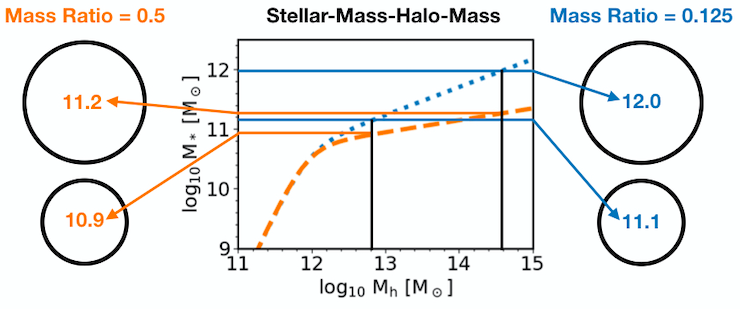
\includegraphics[width = \linewidth]{Figures/Chapter5/MassRatioCartoon.png}
	\caption{A cartoon showing the how the SMHM relation can impact the stellar mass ratio of galaxies mapped into identical halos. The steeper SMHM relation creates a smaller stellar mass ratio as the change in halo mass maps to a much larger stellar mass difference.}
	\label{fig:Mass_Ratio_Toon}
\end{figure}

\begin{figure}[h]
	\centering
	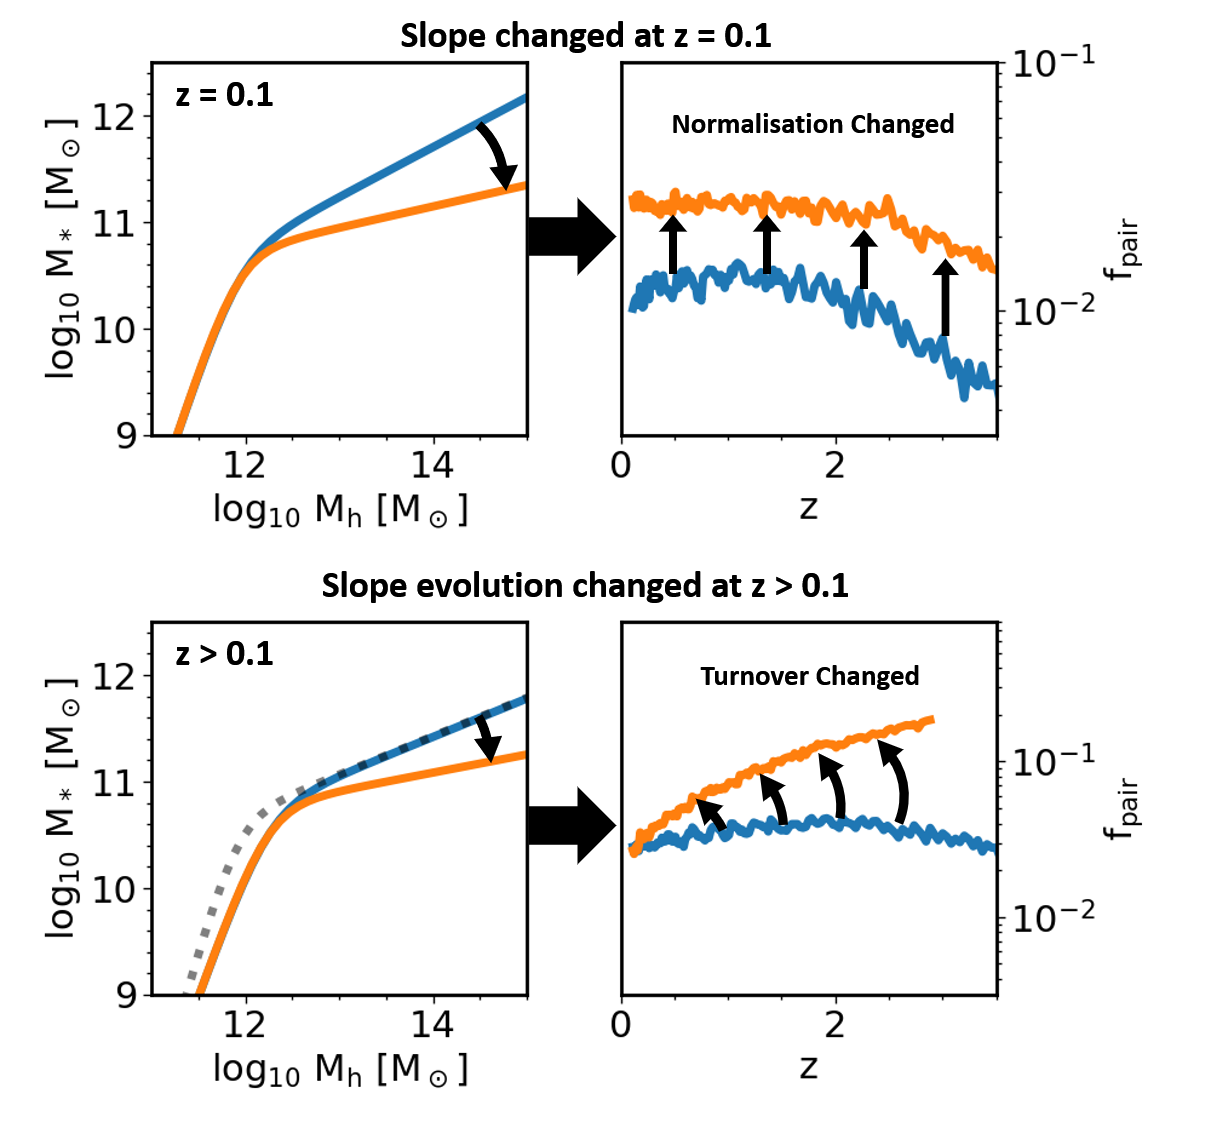
\includegraphics[width = \linewidth]{Figures/Chapter5/SMHM_PF_Cartoon.png}
	\caption{A cartoon showing the how the SMHM relation can impact the pair fraction. The top row shows how reducing the high mass slope of the SMHM relation increase the number of pairs at all redshifts. The bottom row shows the redshift $z=0$ relation as a grey dotted line, two relations at redshift where the relation is not evolved or evolved to be shallower are shown in blue and orange respectively. For this evolving SMHM relation the pair fractions are found to increase. In each case the reason for the increase can be explained by referencing Figure \ref{fig:Mass_Ratio_Toon} where making the relation shallower seeds more massive pairs.}
	\label{fig:Pair_Fraction_Toon}
\end{figure}

\begin{landscape}
\begingroup
\begin{figure}[h]
	\centering
	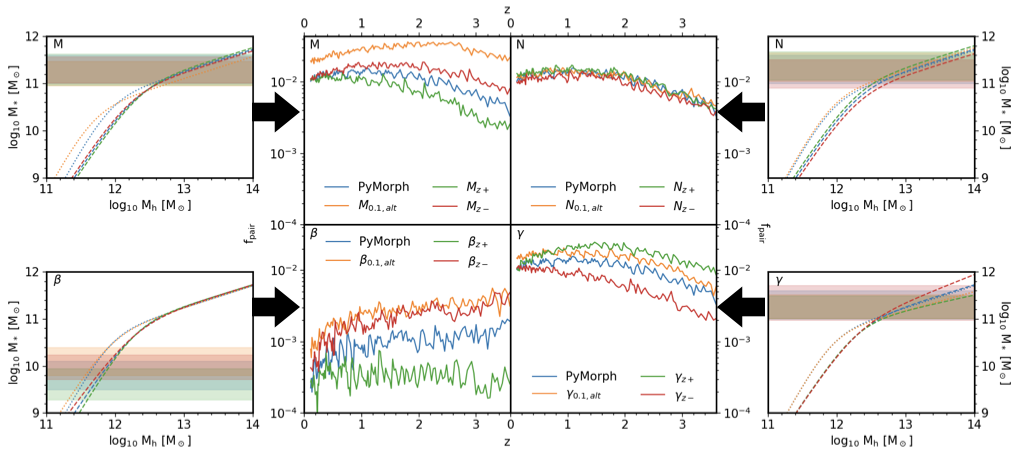
\includegraphics[width = \linewidth]{Figures/Chapter5/PairFractionSystematic.png}
	\caption{Each of the panel pairs (M, N, $\beta$, $\gamma$) shows the input SMHM relation in the outer plot and the modelled pair fraction evolution in the center plot. Each pair investigates adjustments to the given parameter of the SMHM relation (M, N, $\beta$, $\gamma$). Each pair shows the reference SMHM relation `G18' in blue, the relation adjusted at redshift $z = 0.1$ keeping the same SMHM relation evolution parameters in yellow. The red and green lines have the evolution parameter altered such that the evolution parameter is increased or decreased with respect to PyMorph respectively. In the outer (SMHM relation) plots dotted lines are $z = 0.1$ relations and dashed lines are $z = 2$ relations the PyMorph relation is shown at both epochs for comparison. Finally the shaded bands in the outer plots show the consistent number density selections used in the center plots.}
	\label{fig:Pair_Frac_Sys}
\end{figure}
\endgroup
\end{landscape}

\section{Galaxy Morphologies Resulting from Galaxy Mergers}
%What is a galaxy merger and how is it defined?
%how do we estimate the rate of galaxy mergers?
%What happens during a galaxy merger?
%The fraction of elliptical galaxies stemming from galaxy major merger in steel

\begin{figure}[h]
	\centering
	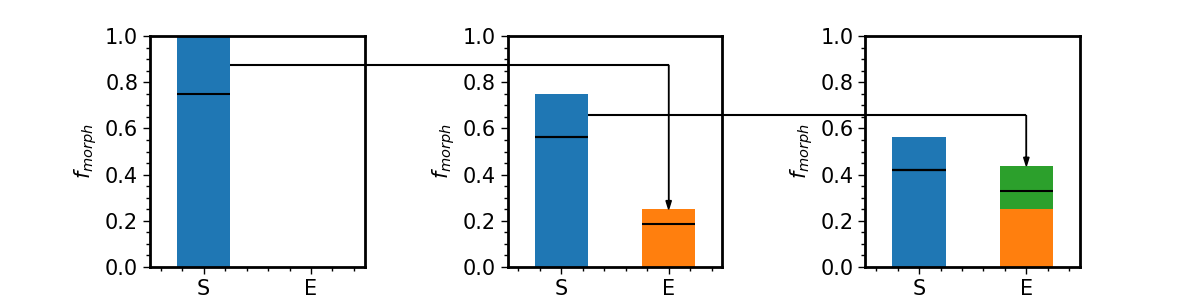
\includegraphics[width = \linewidth]{Figures/Chapter5/Morphology_Evolution.png}
	\caption{A cartoon of the way we assign morphologies statistically in $\steel$. Each step has the same fraction of major mergers but the number of ellipticals created reduces as some major mergers occur on the elliptical fraction. The fraction of galaxies in each population experiencing a major merger is displayed as a horizontal black line.}
	\label{fig:Gal_Morph}
\end{figure}

\begin{figure}[h]
	\centering
	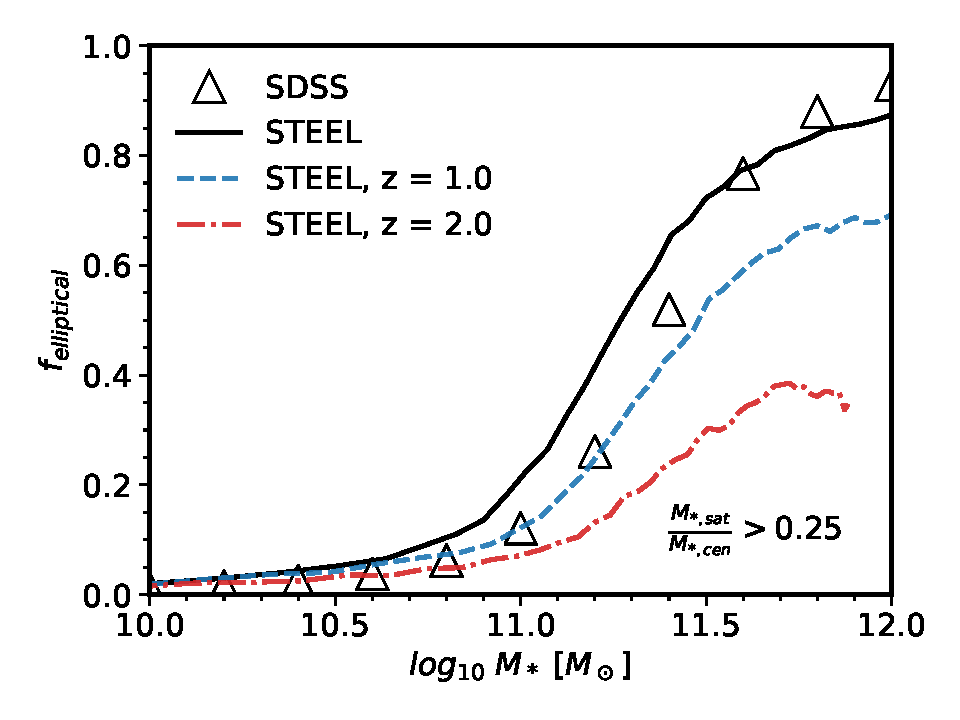
\includegraphics[width = \linewidth]{Figures/Chapter5/GalaxyMorphologies.pdf}
	\caption{I show at three redshift steps the predicted fraction of ellipticals as a function of stellar mass. The lines are the predictions from \textsc{steel} and the triangles are the T-Type selected elliptical fraction from SDSS at redshift $z = 0.1$.}
	\label{fig:Gal_Morph}
\end{figure}


\section{Lenticular Galaxy Formation}
%What is a lenticular and why are they considered independently to the rest of the galaxy population?
%What have been the proposed models of Lenticular formation?
%Building a least assumption model of lenticular formation (supervised project)